\documentclass[3p,12pt]{elsarticle}
\usepackage{amsmath}
\usepackage{here}
\usepackage{caption}
\usepackage{subcaption}
\usepackage{color}
\def\spe{\mathbf{Spec}}
\usepackage{graphicx}
\usepackage{soul}           %package for highlight
\newcommand{\noop}[1]{}
\newtheorem{problem}{Problem}
\usepackage{lineno,hyperref}
\modulolinenumbers[5]
\journal{Mechanical Systems and Signal Processing}
\usepackage{multirow}


%% `Elsevier LaTeX' style
%\bibliographystyle{abbrvnat}%\biboptions{sort&compress}
\bibliographystyle{elsarticle-num}\biboptions{sort&compress}
%%%%%%%%%%%%%%%%%%%%%%%

\begin{document}

\begin{frontmatter}

\title{Separation of multiple local-damage-related components from vibration data using Nonnegative Matrix Factorization and multichannel data fusion}


%% Group authors per affiliation:
\author[label1]{Jacek Wodecki \corref{cor1}}
\cortext[cor1]{Corresponding author, jacek.wodecki@pwr.edu.pl}
\author[label1]{Anna Michalak}
\author[label1]{Rados{\l}aw Zimroz}
\author[label2]{Agnieszka Wy{\l}oma{\'n}ska}

\address[label1]{Faculty of Geoengineering, Mining and Geology, Wroclaw University of Science and Technology, Na Grobli 15, 50-421 Wroclaw, Poland
\\\{jacek.wodecki, anna.michalak radoslaw.zimroz\}@pwr.edu.pl\\}
\address[label2]{Faculty of Pure and Applied Mathematics, Hugo Steinhaus Center, Wroclaw University of Science and Technology,Wybrze{\.z}e Wyspia{\'n}skiego 27, 50-370 Wroclaw, Poland
\\ agnieszka.wylomanska@pwr.edu.pl\\}

\begin{abstract}
The problem of local damage detection in case of analyzing vibration signal from rotating machines is mostly related to the detection of periodic impulsive components. Depending on various features of the signal, this task can be relatively simple in some cases (e.g. for an impulsive component in the presence of Gaussian noise). However, in our case multiple impulsive components occupying with the overlapping frequency bands are present. For all components, the impulses can be periodic. In this article, authors present a novel methodology based on data fusion from multichannel vibration data from heavy-duty industrial gearbox operating in the driving station of a belt conveyor. The proposed method is based on the factorization of spectrograms using Generalized Hierarchical Alternating Least Squares Nonnegative Matrix Factorization with Beta-Divergence (later referred to as $\beta$-HALS NMF). Partial information obtained from the factorization is fused into a single data set for each impulsive component present in the signal. Finally, Griffin-Lim algorithm is used to estimate the complex phase layer of artificial spectrograms allowing to recover the near-perfect time series of each impulsive component extracted from the signal. This method has been tested on four-channel vibration data.
\end{abstract}

\begin{keyword}
Nonnegative Matrix Factorization, beta-divergence, local damage detection, time-frequency representation, phase reconstruction, data fusion, vibration
\end{keyword}

\end{frontmatter}

\linenumbers

\section{Introduction}

Local damage detection is still a relevant topic in condition monitoring machines with rotating components. Solutions described in the literature are able to detect damage in rolling element bearings or gearboxes, even if impulsive component related to the damage has low energy and is hidden in the vibration data \cite{samuel2005review,randall2011rolling}. Typically methods are focusing on detection of impulsive properties of the so-called signal of interest (SOI) \cite{antoni2006spectral,wodecki2018optimal,zak20161932,obuchowski2014selection} or cyclic/periodic character of SOI \cite{cioch2013finding}. Although the effectiveness of such methods is substantial, there are still challenges in this area. One of them is the fact that operating conditions are time-varying. In this case, both cycle length, as well as the amplitude of impulses, might be load/speed dependent \cite{gryllias2018application}.

A significant amount of~research conducted in~recent years was aimed at~fault detection in~the~presence of~Gaussian noise. Antoni and Randall have put forth very interesting approach based on~very simple statistic \cite{antoni_randall}. This presents a~detection method using the spectral extension of~the~sample kurtosis. In such a~way, it~can represent a~filter magnitude characteristics that can be used to perform filtration on an input signal, which will expose the impulsive behavior hidden within.

One of the recent concepts for local damage detection based on the vibration data has been presented by {\.Z}ak et al. where authors investigate the possibility of constructing a selector based on the $\alpha$ parameter of the $\alpha$-stable distribution \cite{zak20161932}. As an indicator of distance from Gaussian distribution, the $\alpha$-based selector can identify frequency bands containing impulsive behaviors, and it can serve as a convenient preprocessing tool. Authors of \cite{zak2019periodically} also tried to apply fractional lower-order covariance as a base for constructing a novel lag-frequency map, that allows analyzing the periodic signals.

Continuing the idea of pattern recognition based on the multidimensional data representations, one could observe the increasing interest in matrix factorization techniques applied to multidimensional data structures. Following this direction, the approach of Nonnegative Matrix Factorization (NMF) gains popularity in recent years \cite{cichocki2009nonnegative,lee1999learning,zdunek2008data}. This class of algorithms is especially suitable for the analysis of the representations describing energy distribution (e.g.spectrogram) because by definition, they contain only the nonnegative values. Following this idea, Wodecki et al. proposed a collection of methods for local damage detection based on the factorization of time-frequency and bi-frequency representations \cite{wodecki2017local,wodecki2019novel,wodecki2019impulsive}.

In this paper, the authors present a technique for the identification and extraction of multiple cyclic components from the multichannel vibration data. The described method is based on the factorization of spectrogram matrices calculated for each channel, which allows analyzing the occurring patterns. Detected information about the individual components is then extracted from each channel and merged, which allows to reconstruct and separate the components and transform them back into the time domain. 


\subsection{Problem formulation}


From the point of view of data analysis, the problem of vibration-based local damage detection can become very difficult in the presence of disadvantageous circumstances. Typically local damage is identified based on the presence of the cyclic (or even periodic) impulsive component in the diagnostic signal. In the simplest scenario, the input data contains only one impulsive component related to the local damage, and the remaining components of the signal are stationary. In such a case, the techniques that aim towards the maximization of the impulsiveness of nonstationarity can be very successful in defining informative frequency band for the filter construction, and in consequence extract the component of interest \cite{combet2009optimal,wodecki2017local}. 

A different situation occurs when the damage-related component has to be identified in the presence of a nonstationary or even impulsive noise, which is obviously non-Gaussian \textcolor{red}{(which is not the case in the example presented in this paper)}. In such a case, impulsiveness-related methods become inappropriate, as they become sensitive to the impulsive noise, which might be much more energetic than the cyclic component of interest \cite{wodecki2019novel,wylomanska2016impulsive,tran2001method}. In such a scenario it is necessary to recognize the fault-related component as a distinct pattern, or even employ cyclostationarity-analysis techniques to focus on the periodic nature of the signal of interest (SOI), rather than the impulsive character of the noise, that is non-periodic \cite{antoni2004cyclostationary}.

The challenging case occurs when multiple cyclic impulsive components are present in the signal. In such case methods such as Spectral Kurtosis \cite{antoni2007cyclic,antoni2006spectral} or other selector-based techniques fall apart \cite{obuchowski2014selection,WYLOMANSKA201714,BARSZCZ2011431,protrugram_PK}, since they cannot differentiate the components and very often build the features common for all of them. At this point, single-dimensional descriptors cannot separate the components. For example, time-domain analysis observes impulses originating from both components however, cannot tell the difference between their sources and can only interpret them as a single non-cyclic impulsive component. On the other hand, frequency-domain analysis can reveal the spectral structure of each component but is not capable of separating the patterns from the mixture of the individual spectra, and as a consequence builds the common features for them.

The solution to this problem lies in the multidimensional analysis. The critical aspect is the appropriate domain selection. One of the time-frequency representations would be the most straightforward choice. However, it is important to remember that windowing imposes resolution constraints, and components characterized by the higher frequency of modulations may not be represented correctly in the time domain. In such cases, it is recommended to use bi-frequency maps or other types of multidimensional data representation.

The rest of this paper is organized as follows: in section \ref{meth} main concepts of used tools are explained, after that the simulation procedure and obtained results are presented. Next, in section \ref{disc} main concerns regarding the usage of the presented method are discussed and finally, the conclusions are formulated. 


\section{Methodology}\label{meth}

\begin{table}[ht!]
    \centering
    \caption{List of symbols of variables}
    	\resizebox{\textwidth}{!}{
    \begin{tabular}{|l|l|}
    \hline
         \textbf{Notation} & \textbf{Definition} \\ \hline
         \textit{M} & Number of input channels within a multichannel time series data\\ \hline
         \textit{N}  & Number of data samples in time series of each channel \\ \hline
         \textbf{S}$^{N\times M}$ & M-dimensional input signal in the form of time series\\ \hline
         $\mathbf{s}_m= (s_1^{(m)},\dots,s_N^{(m)}) $ & Time series of a single input channel (column vector of matrix \textbf{S})  \\ \hline
         \textit{I}  & Number of spectrogram frequency bins \\ \hline
         \textit{K}  & Number of spectrogram time points \\ \hline
         \textbf{Y}$^{I\times K}$ & Spectrogram matrix \\ \hline
         \textit{J}  & Number of NMF classes \\ \hline
         \textbf{A}$^{I\times J}$ & NMF base matrix \\ \hline
         $\mathbf{X}^{K\times J} =\mathbf{B}^\textrm{T}$ & NMF encoding matrix \\ \hline
         $\mathbf{b}_j^\textrm{T}$ & Single encoding component\\ \hline
         \textbf{E}$^{I\times K}$ & Error matrix in NMF optimization process \\ \hline
         $\beta^{1\times1}$ & Parameter for divergence definition \\ \hline
         \textit{h}  & Output class indicator \\ \hline
         \textbf{C}$^{M\times J}$ & Component identification dictionary matrix \\ \hline
         $\mathbf{\widetilde{A}}^{I\times M}$ & Estimated base matrix for an individual output component \\ \hline
         $\mathbf{\widetilde{X}}^{M\times K}$ & Estimated encoding matrix for an individual output component \\ \hline
         $\mathbf{\widetilde{Y}}^{I\times K}$ & Estimated spectrogram matrix for an individual output component \\ \hline
         $\mathbf{\widehat{Y}}^{I\times K}$ & Estimated STFT matrix for an individual output component \\ \hline
    \hline
    \end{tabular}
    }
    \label{tab:tab2}
\end{table}

In this section, the authors describe the details of the presented approach. The aim is to identify, separate, and extract individual components describing different faults within the machine, assuming that both of them are impulsive and periodic. For improved readability the utilized notation is presented in Table \ref{tab:tab2}.

The proposed procedure consists of three main stages:

\begin{itemize}
    \item \textbf{Preprocessing -} this stage consists of the steps needed for preparing the appropriate data structures for the actual exploratory analysis. First, for time series of each raw input channel, a spectrogram is calculated (section \ref{sec_spec}). Next, each of those is factorized using $\beta$-HALS NMF algorithm, which produces two feature matrices (called \emph{base} and \emph{encoding} matrices) for each channel (section \ref{nmf}).
    \item \textbf{Selection -} at this stage, information is identified and classified. Vectors of feature matrices from all channels are assigned to one of the classes based on the analysis of encoding matrices (section \ref{ident}). When all features are labeled, they are pulled from the matrices and assembled into new feature matrices for each class respectively (section \ref{rec}).
    \item \textbf{Recovery -} at this stage, the individual components are reconstructed. For each class its specific spectrogram is estimated by multiplying base and encoding matrices according to the NMF model (eq. (\ref{eq:NMF})). Then, the complex phase is estimated for the obtained spectrograms using Griffin-Lim algorithm (section \ref{gla}). This way it is possible to transform the spectrograms back to the time series, which produces the reconstructed signal components.
\end{itemize}

For the presented procedure the input data is provided in the form of multichannel vibration signal $\mathbf{S}=[\mathbf{s}_1,\dots,\mathbf{s}_M]$ where $M$ is the number of input channels.

\subsection{Stage 1: Preprocessing}

\subsubsection{Spectrogram}\label{sec_spec}

Short-time Fourier transform (STFT), which for one-dimensional discrete data $\mathbf{s}_m= (s_1^{(m)},\dots,s_N^{(m)})$, with $m\in1,\dots,M$, is given by the formula \cite{allen1977short}:

\begin{equation}
    \textrm{STFT}(i,k)=\sum_{f=0}^{L-1}s[k+f]w[f]e^{-j2\pi if/I},
\end{equation}
where $j$ is the imaginary operator, $0\leq i \leq I-1$ is frequency bin for the $I$ total frequency bins, $k=0,\dots,K-1$ is time point for the $K$ total time points, and $w[.]$ is the window of length $L$. One can observe that in STFT for each time point the Fourier Transform is calculated using Fast Fourier Transform (FFT). Furthermore, the spectrogram is an absolute value of the STFT:

\begin{equation}
\label{eq:spec_Y}
Y(i,k)=\textrm{Spec}(i,k)=|\textrm{STFT}(i,k)|.
\end{equation}


\subsubsection{Generalized Hierarchical Alternating Least Squares Nonnegative Matrix Factorization with Beta-Divergence}\label{nmf}
The next step of the proposed procedure is the factorization of spectrograms for each channel for internal feature analysis. Nonnegative Matrix Factorization is a broad class of matrix factorization algorithms that can be characterized with very characteristic common feature: input matrix, as well as all output matrices, do not contain negative values. Because of that, they are suitable as a tool for the analysis of energy-based data representations. The described NMF procedure is defined for the single spectrogram factorization and is performed for each channel separately.

In this paper, we consider the NMF model given by \cite{cichocki2009nonnegative}:

\begin{equation}
   \label{eq:NMF} 
   \mathbf{Y}=\mathbf{AX}+\mathbf{E} = \mathbf{AB}^\textrm{T} +\mathbf{E},
\end{equation}
where the known non-negative input spectrogram matrix $\mathbf{Y}=[y_{ik}] \in \mathbb{R}^{I\times K}$, defined in equation (\ref{eq:spec_Y}), is approximated by the product of unknown matrices: $\mathbf{A} = [\mathbf{a}_1, \dots, \mathbf{a}_J] \in \mathbb{R}_+^{I\times J}$ which is the base matrix with non-negative vectors $\mathbf{a}_j$, and $\mathbf{X}=\mathbf{B}^\textrm{T} = [\mathbf{b}_1,\dots, \mathbf{b}_J]^\textrm{T} \in \mathbb{R}_{+}^{K\times J}$ that represents the non-negative components $\mathbf{b}_j^\textrm{T}$ ($j=1,\dots,J$, where $J$ is the number of NMF classes) with $\mathbf{E}=[e_{ik}] \in \mathbb{R}^{I \times K}$ containing the errors or noise. As non-negative matrices or vectors, we understand that each element of these matrices or vectors are equal to or bigger than 0. 

In this case, to obtain the particular configuration of the algorithm, we use a set of local cost functions Beta-divergences and perform simultaneous or sequential (one-by-one) minimization of these local cost functions. These algorithms are suitable for a large scale dataset because of the fast processing speed and the local nature of the learning rules \cite{cichocki2008flexible,cichocki2009fast}.
The Beta-divergence ($D_\beta(\cdot||\cdot)$) cost function between two nonnegative sequences is defined as follows:
\begin{equation} 
\label{eq:beta_equations}
   D_\beta^{(j)}([\mathbf{Y}^{(j)}]_{+} ||\mathbf{a}_j\mathbf{b}_j^\textrm{T})=
\begin{cases}
\sum_{ik} \left(y_{ik}^{(j)} \frac{\left[y_{ik}^{(j)}\right]^\beta - \left[q_{ik}^{(j)}\right]^{\beta}}{\beta} - \frac{\left[y_{ik}^{(j)}\right]^{\beta+1} - \left[q_{ik}^{(j)}\right]^{\beta + 1}}{\beta+1}    \right), \quad \beta>0,\\
\sum_{ik} \left(y_{ik}^{(j)} \ln \left(  \frac{y_{ik}^{(j)}}{q_{ik}^{(j)}} \right) -y_{ik}^{(j)}+q_{ik}^{(j)}   \right), \quad \beta=0,\\
\sum_{ik} \left(  \ln \left(  \frac{q_{ik}^{(j)}}{y_{ik}^{(j)}}  \right)   + \frac{y_{ik}^{(j)}}{q_{ik}^{(j)}}  -1 \right),   \quad \beta=-1,
\end{cases}
\end{equation}
where $y_{ik}^{(j)} = \left[ y_{ik} - \sum_{p\neq j} a_{ip}b_{kp} \right]_{+}$ and $q_{ik}^{(j)} = \hat{y}_{ik}^{(j)} = a_{ij}b_{kj}$ for $j=1,\dots,J$. Selection of the $\beta$ parameter is based on the statistical distribution of the data. The Beta-divergences are inherently tied to Tweedie models \cite{Tweedie}. The optimal choice of the $\beta$ parameter for different error or noise (represented by the matrix $\mathbf{E}$ in eq. (\ref{eq:NMF})) distribution is presented in Tab. \ref{tab:beta_parameter}. 

\begin{table}[!ht]
    \centering
        \caption{The optimal choice of the $\beta$ parameter in case of the different noise distribution.}
    \begin{tabular}{l|c}
        Distribution & $\beta$ parameter \\ \hline
         Gaussian& 1 \\
         Poisson & $0$ \\ 
         compound Poisson & $(-1,0)$ \\
         Gamma & $-1$ \\
    \end{tabular}
    \label{tab:beta_parameter}
\end{table}

The columns of $\mathbf{E}=[\mathbf{e}_1,\dots,\mathbf{e}_K]$ in model (\ref{eq:NMF}) are the vectors of independent identically distributed random variables with the mean value $\mu(\mathbf{e}_k)=0$ and covariance matrix $\Sigma_\mathbf{E} \in \mathbb{R}_+^{I\times I}$. The matrix $\mathbf{E}$ can be described with the joint Gaussian distribution \cite{tong2012multivariate}:

\begin{equation}
    \frac{1}{\left((2\pi)^I\mathrm{det}\{\Sigma_\mathbf{E}\} \right)^{\textrm{T}/2}}exp\left\{-\frac{1}{2}\mathrm{tr}(\mathbf{E}^\textrm{T}\Sigma_\mathbf{E}^{-1}\mathbf{E}) \right\}.
\end{equation}


To obtain the multiplicative learning algorithm, we calculate the gradient (\ref{eq:beta_equations}) with respect to the elements $a_{ij}$ and $b_{kj}$. Next, we equate obtained gradient components to zero to get the simple Hierarchical Alternating Least Squares (HALS) update rules \cite{cichocki2009nonnegative} referred to as the HALS with $\beta$-divergence. These update rules can be represented in a generalized compact vector form as: 

\begin{equation}
   \label{eq:beta_up_rules} 
   \mathbf{b}_j \leftarrow \frac{\left( \left[\mathbf{Y}^{(j)\textrm{T}} \right]_{+}\right)\Psi (\mathbf{a}_j) }{\Psi (\mathbf{a}_j^\textrm{T})\mathbf{a}_j}, \quad \quad a_j \leftarrow \frac{\left( \left[\mathbf{Y}^{(j)} \right]_{+}\right)\Psi (\mathbf{b}_j) }{\Psi (\mathbf{b}_j^\textrm{T})\mathbf{b}_j},  \quad (j=1,\dots,J),
\end{equation}
where $\Psi(\mathbf{b})$ is a suitably chosen convex function, and all nonlinear operation are performed element-wise.

The approach presented in this paper is one of the special cases. The optimal $\beta$ parameter based on Tab. \ref{tab:beta_parameter} is 1 (under the assumption of the Gaussianity of the noise) and the convex function is $\Psi(\mathbf{b})=\mathbf{b}^{.\beta}$, where rise to the power $\beta$ is performed element-wise. 
\subsection{Stage 2: Selection}
\subsubsection{Class identification}\label{ident}

The identification process is performed based on the kurtosis value of component vectors in encoding matrices (matrices denoted as $\mathrm{\mathbf{X}}^{\{j\}}$, $j=1,\dots,J$). The kurtosis has been chosen as a criterion because the fault components are expected to be impulsive in opposition to the noise component which will remain quasi-Gaussian. The kurtosis very often is considered as the measure of impulsiveness (it measures the distance from Gaussian distribution). The kurtosis of any univariate Gaussian distribution is 3. If the distribution has kurtosis higher than 3, it means that the outliers (impulses) in data are observed \cite{decarlo1997meaning}.

NMF allows to differentiate components describing particular faults from each other as well as from the noise. Authors assume that all of those are present in all input channels, and hence will appear as a class after factorization for each channel. As a result, after factorizing each of $M$ channels into $J$ classes, $M\times J$ components are obtained, that need to be identified. Each fault component is expected to have a different value of kurtosis, because they have different frequencies of impulse occurrence (in practice different amount of impulses per signal length). As a result of such an assumption, it is expected that components can be classified into $J$ classes, each with different average kurtosis value. 

The simplest way to achieve that is to define thresholds separating those classes in terms of the kurtosis value, which is defined as follows \cite{joanes1998comparing}:
\begin{equation}
\label{eq:kurtosis}
kurt_{\mathbf{x}^{\{m\}}_j}=\frac{\frac{1}{K} \sum_{k=1}^{K} \left(x^{\{m\}}_{jk} - \overline{\mathbf{x}}^{\{m\}}_j \right)^4}{\left({\frac{1}{K} \sum_{k=1}^{K} \left(x^{\{m\}}_{jk} - \overline{\mathbf{x}}^{\{m\}}_j \right)^2}\right)^2}\quad j=1,\dots,J, \quad m=1,\dots,M,
\end{equation}
where the denominator is the second sample central moment squared (sample variance) and the numerator is the fourth sample central moment. This way $x^{\{m\}}_{jk}$ is the $k^{th}$ sample of the $j^{th}$ component vector from the encoding matrix describing the $m^{th}$ channel and $\overline{\mathbf{x}}^{\{m\}}_j$ is the mean of the $j^{th}$ component vector from the encoding matrix describing the $m^{th}$ channel.

Firstly, the threshold that separates noise from fault components is defined. Because of using a sample estimator to calculate the value of kurtosis of the encoding vectors, for a limited amount of samples available in those vectors the kurtosis value is prone to a significant error. Since the kurtosis value of the noise is in theory equal to 3, authors define the threshold as $T_{noise}=3.5$.


% Firstly, the threshold that separates noise from fault components can be defined as distance of $3\sigma$ from the expected noise kurtosis, such as:

% \begin{equation}
%     T_{noise}=kurt_{noise}+3\textbf{\sigma_{noise}}
% \end{equation}
% where $kurt_{noise}=3$ since the noise component is expected to be quasi-Gaussian, and $\sigma_{noise}$ is the standard deviation of the sample kurtosis \cite{joanes1998comparing}
% \begin{equation}
%     \sigma_{noise}=\sqrt{\frac{24K(K-1)^2}{(K-3)(K-2)(K+3)(K+5)}},
% \end{equation}
% where $K$ is a number of observation in the analyzed vector. 

When noise features are identified, the remaining $J-1$ target components need to be classified (in practice - separated from each other), which is performed by calculating thresholds that separate them. Those thresholds are defined in terms of the modulation frequencies of encoding components. 

The fundamental modulation period of the encoding component is calculated as an averaged distance in time between the positions of consecutive local maxima in the encoding component calculated using Matlab built-in function \texttt{findpeaks}. Fundamental modulation frequency of the component is the inverse of the period value.

When the fundamental modulation frequency is calculated for each encoding component present for the data set (omitting the components already classified as noise), $J-1$ distinct values are expected to emerge (total amount of classes without the noise class). The mean value of two consecutive frequency values determines the threshold that allows to separate the classes described by the regarded frequencies.

% selekcja do C

After classifying components based on the described thresholds authors construct the assignment matrix $\mathbf{C}^{M\times J}$ such as

\begin{equation}
\label{def_C_matrix}
   C_{m,j}=h, 
\end{equation}
where $h\in 1,\dots,J$ indicates the assignment of the $j^{th}$ vector from the base and encoding matrices of $m^{th}$ channel to $h^{th}$ class. 

In this context, it is important to distinguish the meaning of the indices $j$ and $h$. While $j$ iterates the input classes (for factorizing initial spectrograms), $h$ iterates the output classes (reconstructed components). While in the analysis of the example data presented in this article the number of input classes match the number of output classes (hence authors state that $h\in 1,\dots,J$ for simplicity of notation), it is not always the case. 

\subsubsection{Construction of base and encoding matrices}\label{rec}

When all components within each channel are properly assigned into classes, vectors are selected following the information contained in matrix $\mathbf{C}$ (defined in equation (\ref{def_C_matrix})) to construct new base matrix $\widetilde{\mathbf{A}}=[\widetilde{\mathbf{a}}_1,\dots,\widetilde{\mathbf{a}}_M]$ and encoding matrix $\widetilde{\mathbf{X}}=[\widetilde{\mathbf{x}}_1,\dots,\widetilde{\mathbf{x}}_M]^\textrm{T}$ for each component $j$:
\begin{equation}
    \widetilde{\mathbf{a}}^{\{h\}}_m= \mathbf{a}^{\{m\}}_j, \quad \textrm{for} \quad  C_{m,j}=h
\end{equation}
    % Anew_{(j)}[m]=A_{(m)}[:,v]: \exists_{v\in (1,\dots,J)}: A_{(m)}[:,v] \rightarrow C_{(j)}
and
\begin{equation}
    \widetilde{\mathbf{x}}^{\{h\}}_m= \mathbf{x}^{\{m\}}_j, \quad \textrm{for} \quad C_{m,j}=h,
\end{equation}
where $m=1,\dots,M$ is a channel number and $h\in 1,\dots,J$ indicates a particular component.

\subsection{Stage 3: Information recovery}
\subsubsection{Reconstruction of magnitude and phase of the spectrograms}\label{gla}

When the base and encoding matrices are defined for each component, their specific magnitude spectrograms are constructed:

\begin{equation}
    \widetilde{\mathbf{Y}}^{\{h\}}=\widetilde{\mathbf{A}}^{\{h\}}\widetilde{\mathbf{X}}^{\{h\}}, \quad h=1,\dots,J.
\end{equation}

Since the aim is to recover the time series of each component, there is a need to be able to reconstruct the complete complex form representing the STFT, because Matlab build-in function \texttt{istft} takes the complex STFT matrix as input. To achieve this goal, authors propose to perform phase estimation using Griffin-Lim algorithm.

The Griffin-Lim algorithm (GLA) was introduced in 1984 \cite{griffin1984signal}. This is a version of the double-projection algorithm. The problem can be expressed as finding of the complex matrix $\mathbf{\widehat{Y}}^{\{h\}}$ being a complete complex form (later referred to as CCF) of STFT that describes a signal represented by a given nonnegative matrix $\widetilde{\mathbf{Y}}^{\{h\}}$ such that the magnitude of $\mathbf{\widehat{Y}}^{\{h\}}$ is as close as possible to $\widetilde{\mathbf{Y}}^{\{h\}}$.

\begin{equation}
  \min_{\mathbf{\widehat{Y}}^{\{h\}}} = || \mathbf{\widehat{Y}}^{\{h\}} -  P_\mathcal{C}(\mathbf{\widehat{Y}}^{\{h\}}) ||_{\text{F}}^2, \quad \mathbf{\widehat{Y}}^{\{h\}}\in \mathcal{A},
\end{equation}
where $|| \cdot ||_{\text{F}}$ is the Frobenius norm, $\mathcal{C}$ is the set of consistent CCFs, $\mathcal{A}$ is the set of CCFs whose amplitude is the same as the given one. The Frobenius norm of $I$-by-$K$ matrix $\mathbf{\widehat{Y}}^{\{h\}}$ is defined as follows \cite{masuyama2019deep}:

\begin{equation}
 || \mathbf{\widehat{Y}}^{\{h\}} ||_{\text{F}} = \sqrt{\sum_{i=1}^I \sum_{k=1}^K |\widehat{y}^{\{h\}}_{ik}|^2 }.
\end{equation}

By using this algorithm, it is expected to recover the complete complex form (later referred to as CCF) of STFT based on the partial information carried by the magnitude spectrogram. 

\begin{equation}
   \mathbf{\widehat{Y}}^{\{h\}[m+1]} = P_\mathcal{C}(P_\mathcal{A}(\mathbf{\widehat{Y}}^{\{h\}[m]})),
\end{equation}
where $\mathbf{\widehat{Y}}^{\{h\}[m]}$ is a CCF updated through the iteration, $m$ is the iteration index. The metric projections $P_\mathcal{C}$ and $P_\mathcal{A}$ are given by \cite{masuyama2019deep}:

\begin{equation}
   P_\mathcal{C}(\mathbf{\widehat{Y}}^{\{h\}}) = \mathcal{G}(\mathcal{G^\dag}(\mathbf{\widehat{Y}}^{\{h\}}))
\end{equation}

\begin{equation}
   P_\mathcal{A}(\mathbf{\widehat{Y}}^{\{h\}}) = \textbf{Amp} \odot \mathbf{\widehat{Y}}^{\{h\}} \oslash |\mathbf{\widehat{Y}}^{\{h\}}|,
\end{equation}
where $\textbf{Amp}$ is the amplitude, $\mathcal{G}$ is STFT, $\mathcal{G^\dag}$ represents the pseudo-inverse of STFT(iSTFT), the operations $\oslash$, $\odot$  are respectively the element-wise division and multiplication. 

Finally, by using the iSTFT procedure, the signal in the time domain is reconstructed from the obtained matrix $\mathbf{\widehat{Y}}^{\{h\}}$.

\section{Application to simulated data}

\subsection{Data simulation procedure}

For the full control over the experiment, the authors decided to simulate the multichannel input signal $\mathbf{S}=[\mathbf{s}_1,\mathbf{s}_2,\mathbf{s}_3,\mathbf{s}_4]$ according to the general model:
\begin{equation}
\label{eq:signal_model}
    \mathbf{S}=\mathbf{Base}+\mathbf{Faults},
\end{equation}
where $Base$ is a signal describing the operation of the healthy machine, and $Faults$ is the collection of all impulsive components describing faults present in the machine. Consequently, $Base$ and $Faults$ signals are also four-dimensional.

% BASE
To obtain the signal $Base$ describing operation of the healthy machine, mentioned in (\ref{eq:signal_model}), authors used previously acquired signals describing the machine in good technical condition.


% To obtain the signal $Base$ describing operation of the healthy machine, mentioned in (\ref{eq:signal_model}), the authors used the autoregressive model with order 119, which is the optimal value obtained by the BIC criterion \cite{schwarz1978}. The autoregressive AR(p) model is defined as follows:
% \begin{equation}
%     X_t = c + \sum_{i=1}^p \psi_i x_{t-i}+ \varepsilon_t,
% \end{equation}
% where $\psi_1,\dots,\psi_p$ are parameters of the AR model, $c$ is a constant and $\{\varepsilon_t\}$ is white noise. For estimating the coefficients we used the Yule-Walker method \cite{yule1927vii,walker1931periodicity}. The AR model for each channel is estimated based on real-life vibration signal measured on a typical gearbox operating in the mining industry. For each channel this signal is different to take into consideration the different response of the system from the point of view of each hypothetical sensor. The modeling was necessary to obtain $Base$ signals that do not contain any unwanted disturbances (e.g. local artifacts), but on the other hand, it allows to use the basis for the input data that is describing the actual machine during operation, especially from the point of view of spectral structure of such signal.

%% FAULT
A single fault component is constructed as a sequence of individual impulses distributed in time with a period corresponding to the modulation frequency $f_{mod}$ of the simulated fault. A single impulse is defined as a decaying harmonic oscillation:

\begin{equation}
    g(t)=A\cdot\sin{(2 \pi f_c t)}e^{-dt},
\end{equation}
where $A$ is the amplitude, $t$ is time, $f_c$ is the center frequency of the carrier band of the impulse and $d$ is a decay factor for the exponential function. Center frequency $f_c$ is defined separately for each of the simulated faults. 

%%
\subsection{Results}

In this section, we examine simulated data, which represents four channel vibration signal from the gearbox. Frequencies that characterize the machine operation are presented in Tab.~\ref{tab: obj_gear}. The particular machine, based on which the simulated signal is prepared, is shown in Fig.~\ref{fig:obj_gear}

\begin{table}[ht!]
	\caption{Gearbox and bearing characteristic frequencies}
	\begin{center}
	\resizebox{\textwidth}{!}{
		\begin{tabular}{|c|c|l|l|l|}
			\hline
			&\textbf{No} & \textbf{Notation} & \textbf{Description} & \textbf{Value/unit} \\ \hline\hline
			\multirow{6}{*}{\rotatebox[origin=c]{90}{\textbf{Gearbox}}}&1 & $f_{01}=\frac{n_1}{60}$ & Rotational freq. of the $1^{st}$ shaft & 16.58 Hz \\ \cline{2-5}
			&\textbf{2} & $f_{02}=\frac{n_2}{60}=\frac{n_1}{60 \cdot u_1}$ & \textbf{Rotational freq. of the $2^{nd}$ shaft} & \textbf{4.1 Hz} \\ \cline{2-5}
			&3 & $f_{03}=\frac{n_3}{60}=\frac{n_1}{60 \cdot u_1 \cdot u_2}$  & Rotational freq. of the $3^{rd}$ shaft & 1.31 Hz \\ \cline{2-5}
			&4 & $f_{z_{12}}=\frac{n_1 \cdot z_1}{60}$ & Gear mesh freq. of the $1^{st}$ stage & 381.42 Hz \\ \cline{2-5}
			&5 & $f_{z_{34}}=\frac{n_2 \cdot z_3}{60}$ & Gear mesh freq. of the $2^{nd}$ stage & 147.6 Hz \\ \cline{2-5}
			&6 & $U_p=\frac{z_2 \cdot z_4}{z_1 \cdot z_3}$ & Ratio & 12.69 \\ \hline\hline
					\multirow{4}{*}{\rotatebox[origin=c]{90}{\textbf{Bearing}}}&	1 & \textcolor{red}{$f_{FTF}=0.5*f_r*(1-d/D)$} & Fundamental train freq. & 0.53 Hz \\ \cline{2-5}
% 		&2 & $f_{BSF}$ & Ball spin freq. & 4.45 Hz \\\cline{2-5}
	&	2 & \textcolor{red}{$f_{BFF}=D/d*f_r*[1-(d/D)^2]$} & Ball fault freq. & 9.1 Hz \\ \cline{2-5}
		&\textbf{3} & \textcolor{red}{\textbf{$f_{BPFO}=n/2*f_r*(1-d/D)$}} & \textbf{Ball passing freq. outer race} & \textbf{12.69 Hz} \\ \cline{2-5}
	&	4 & \textcolor{red}{$f_{BPFI}=n/2*f_r*(1+d/D)$} & Ball passing freq. inner race & 16.51 Hz \\ \hline
		\end{tabular}
		}
	\end{center} 
	\label{tab: obj_gear}
\end{table}

\begin{figure}[ht!]
\centering
\includegraphics[width=0.7\textwidth]{figs/obj_gear.png}
\caption{Two-stage gearbox}
\label{fig:obj_gear}
\end{figure}

\textcolor{red}{The values of frequencies related to the gearbox have been obtained using the formulae presented in Tab. \ref{tab: obj_gear} and parameters of the real-life considered gearbox where numbers of teeth on the gearwheels are respectively $z_1=23, z_2=93, z_3=36, z_4=113$, and the rotational speed of the input shaft is equal to $n1=995$ RPM.}
\textcolor{red}{Similarly, the values of frequencies related to the bearing have been obtained using parameters of the real-life bearing, where diameter of rolling element $d=87$ mm, division diameter $D=665$ mm, nominal rotational speed $f_r=73$ RPM, and number of rotating elements $n=24$.}

Two simulated impulsive components have been selected in such a way that the placement of the frequency band of each component in the carrier frequency domain corresponds to the physical understanding of resonant frequency bands for different types of failures \cite{bartelmus2010modelling}. Consequently, one of the impulsive components describes the local damage of the meshing of the gearwheel on the second shaft ($f_c\sim$ 600 Hz, $f_{mod}=$4.1 Hz), and the other - local damage of the outer race of the bearing of the third shaft ($f_c\sim$ 2 kHz, $f_{mod}=$12.69 Hz). \textcolor{red}{Fig. \ref{fig:imp_specs} presents the spectra of the exemplary impulses from each fault components. It can be seen that while parameterization of the impulsive components had to follow the reality (in particular their center frequencies are not very close to each other), the spectra are overlapping, which typically imposes additional difficulty for simpler analytical techniques.} Consequently, having a base signal and two damage-related components in each input channel, the number of classes for spectrogram factorization has been defined as $J=3$.

\begin{figure}[ht!]
\centering
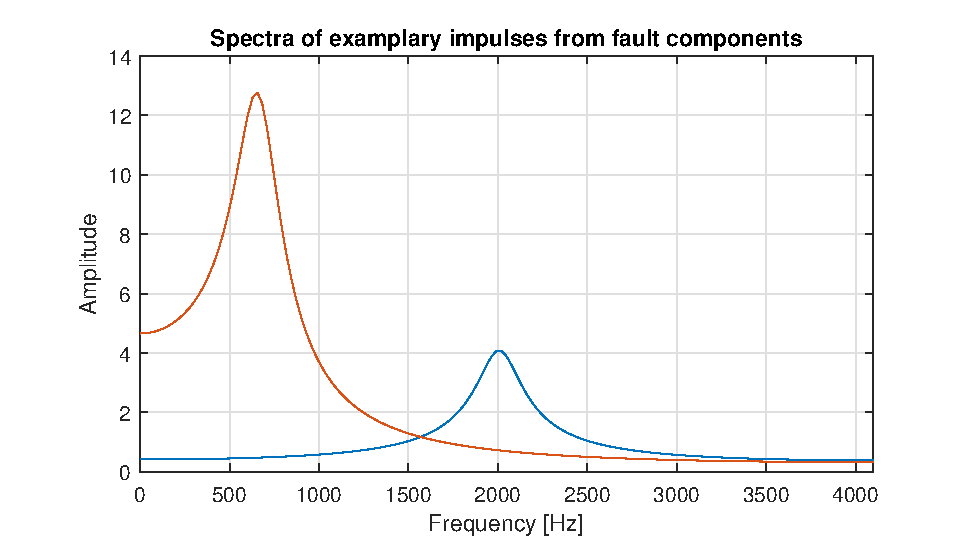
\includegraphics[width=0.8\textwidth]{figs/specs.eps}
\caption{\textcolor{red}{Spectra of the examplary impulses from each fault component. Red line describes the spectrum of the impulse related to the gearwheel damage, blue line - the bearing damage.}}
\label{fig:imp_specs}
\end{figure}



\begin{figure}[ht!]
\centering
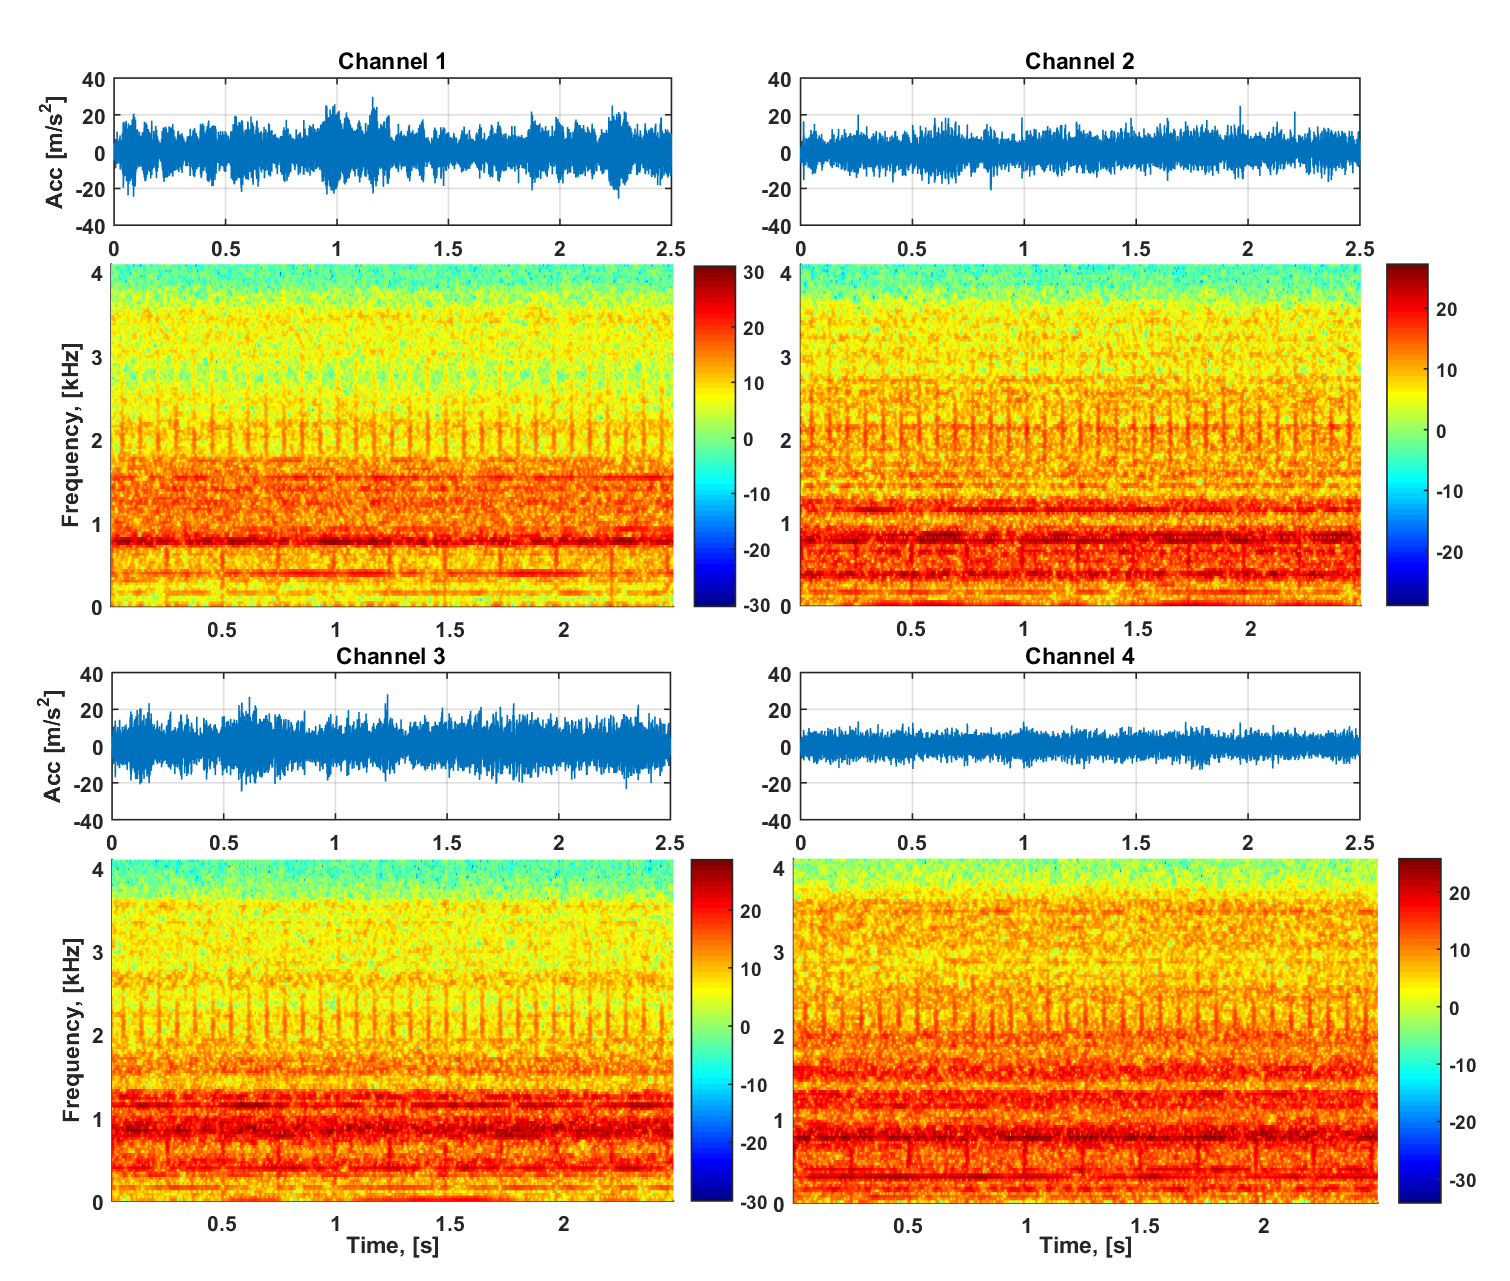
\includegraphics[width=0.8\textwidth]{figs/raw.eps}
\caption{Raw vibration data (top panels) and their time-frequency representations (bottom panels) for each channel.}
\label{fig:raw_signal_all}
\end{figure}

Time series of the individual channels along with the corresponding spectrograms are presented in Fig. \ref{fig:raw_signal_all}. Spectrograms for all channels are calculated identically with the Hamming window of the length equal to 256 samples, 230-sample overlap, and 256-samples long FFT. One can see that time plots do not reveal the presence of any impulsive behavior. However, it can be observed on the spectrograms that the information about the impulsive components is distributed among the channels.


First, each spectrogram is factorized using the $\beta$-HALS NMF algorithm (see section \ref{nmf}).  The output base and encoding matrices for each channel are presented in Fig. \ref{fig:NMF_matrix}.




\begin{figure}[ht!]
\centering
\includegraphics[width=0.8\textwidth]{figs/mats3.eps}
\caption{Base (left panels) and encoding (right panels) matrices for each of four channels with class identification.}
\label{fig:NMF_matrix}
\end{figure}

\begin{figure}[ht!]
\centering
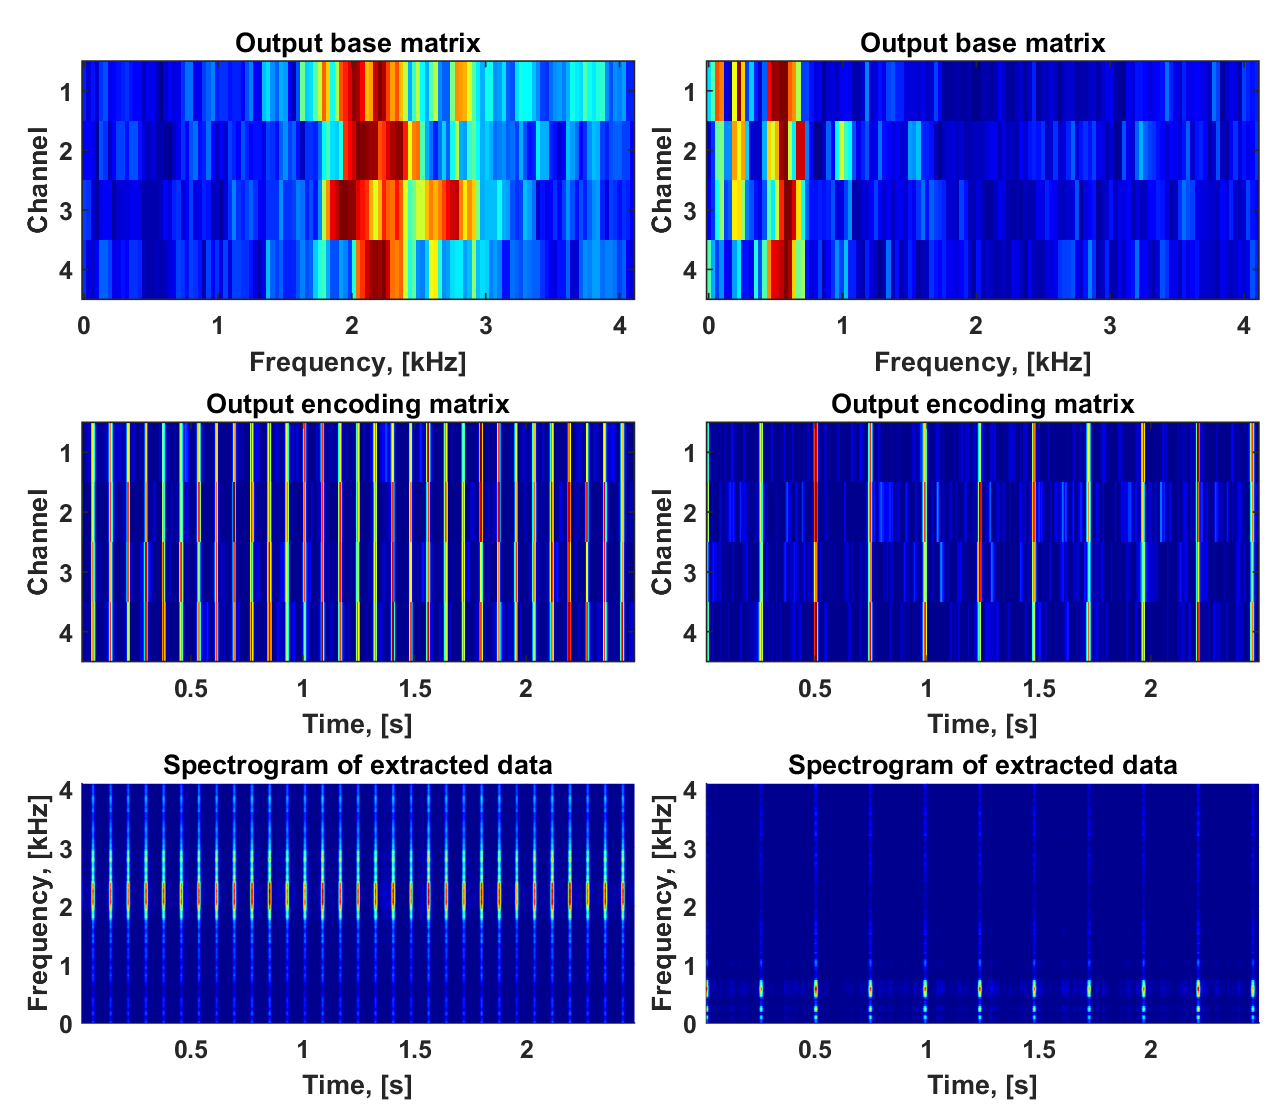
\includegraphics[width=0.8\textwidth]{figs/res.eps}
\caption{Feature matrices reconstructed for both components (top and middle panels) with corresponding recovered magnitude spectrograms (bottom panels).}
\label{fig:NMF_result}
\end{figure}

In the next step feature vectors from the encoding matrices are grouped based on their kurtosis value, which allows identifying distinct classes of behavior. After properly identifying the particular classes, components from the base and encoding matrices are composited into the output base and encoding matrix for each component. After multiplying them, the component-specific magnitude spectrograms are created (see Fig. \ref{fig:NMF_result}). 

\begin{figure}[ht!]
\centering
\includegraphics[width=0.7\textwidth]{figs/out.png}
\caption{Separate components extracted from the signals.}
\label{fig:NMF_out}
\end{figure}

In the next step, Griffin-Lim algorithm allows to estimate the phase layer for the spectrograms, which enables the reconstruction of time series for each impulsive component (see Fig. \ref{fig:NMF_out}). Finally, envelope spectra of recovered components are evaluated to confirm their correct recovery and the presence of harmonics corresponding to the faults \cite{randall2011vibration}.

As a result, both cyclic components have been properly recovered. The value of kurtosis of obtained time series has been chosen as a measure of impulsiveness, and hence the quality of the results. The kurtosis takes the values of 182.78 for the bearing-related fault, and 297.18 for the tooth-related fault.

\begin{figure}[ht!]
\centering
\includegraphics[width=0.7\textwidth]{figs/spec.png}
\caption{Envelope spectra of recovered components.}
\label{fig:spec}
\end{figure}

\subsection{Real-life data analysis}

\textcolor{red}{In this section authors apply the presented method to dual-channel vibration signal measured on similar type of industrial gearbox which was known to experience two types of fault: local damage on the gearwheel on the first shaft, and distributed rather than localized damage of the second shaft (frequencies laid out in the first part of Tab. \ref{tab: obj_gear} apply). Input data is presented in the Fig. \ref{fig:input2}.} 

\begin{figure}[ht!]
\centering
\includegraphics[width=0.8\textwidth]{figs/input2.png}
\caption{\textcolor{red}{Raw vibration data and their spectrograms for dual-channel case.}}
\label{fig:input2}
\end{figure}

\textcolor{red}{Feature matrices after factorizing both spectrograms are presented in Fig. \ref{fig:NMF_matrix2}. Both cyclic behaviors have been properly isolated from the signals, which is easiest visible on the features contained in the encoding matrices. One can observe that base features describing local damage (described as DMG1) indicate broad spectrum as it can be seen on the spectrograms. On the other hand, base feature of distributed damage (DMG2) is mostly focused on the lowest part of the spectrum at about 400 Hz (not to be confused with constant frequency component related to normal machine operation present in all of the base features). After classification and fusing the feature vectors for each class, reconstructed spectrograms with their feature matrices are presented in Fig. \ref{fig:NMF_result2}.} 

\begin{figure}[ht!]
\centering
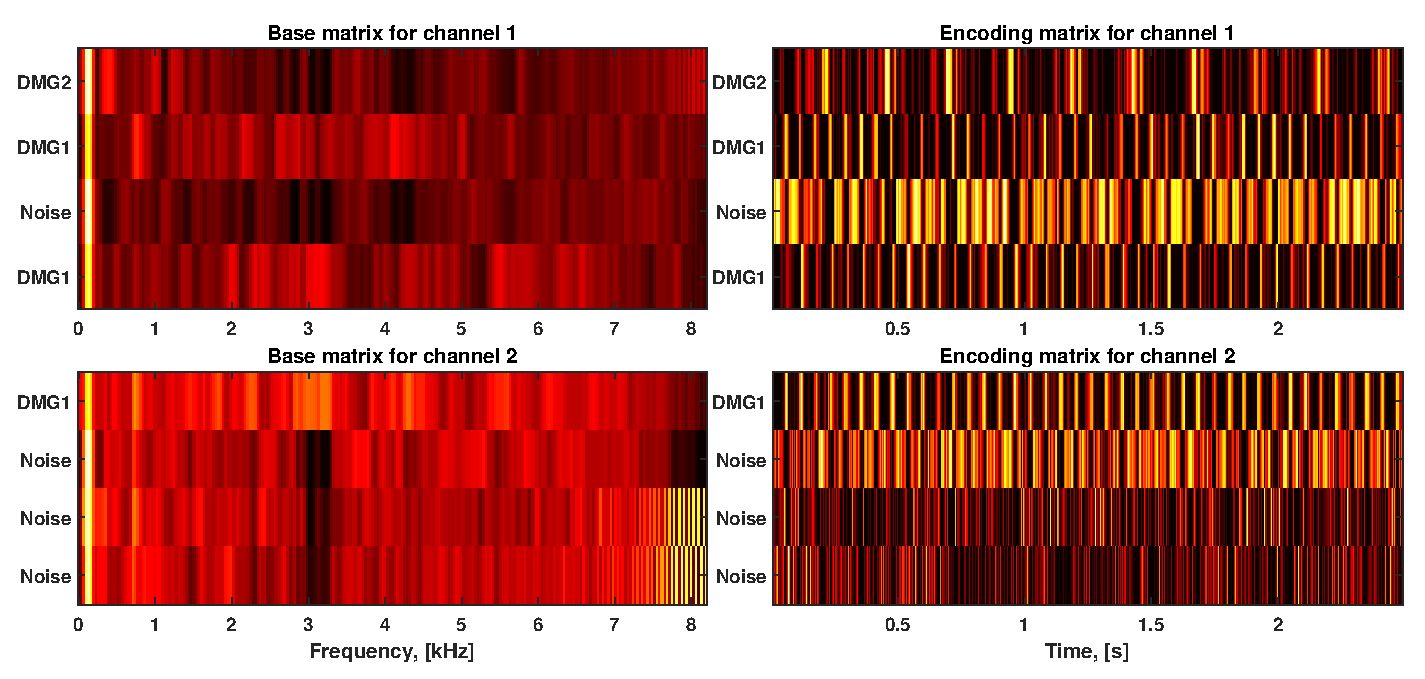
\includegraphics[width=0.9\textwidth]{figs/mats4.eps}
\caption{\textcolor{red}{Base (left panels) and encoding (right panels) matrices for each channel with class identification.}}
\label{fig:NMF_matrix2}
\end{figure}

\begin{figure}[ht!]
\centering
\includegraphics[width=0.9\textwidth]{figs/feat2.png}
\caption{\textcolor{red}{Feature matrices reconstructed for both components (top and middle panels) with corresponding recovered magnitude spectrograms (bottom panels).}}
\label{fig:NMF_result2}
\end{figure}

\textcolor{red}{Finally, reconstructed time series of both components are presented in Fig. \ref{fig:NMF_out2}. Their envelope spectra displayed in the Fig. \ref{fig:NMF_env2} confirm the frequencies related to the suspected machine elements.}

\begin{figure}[ht!]
\centering
\includegraphics[width=\textwidth]{figs/res2.png}
\caption{\textcolor{red}{Separate components extracted from the signals.}}
\label{fig:NMF_out2}
\end{figure}

\begin{figure}[ht!]
\centering
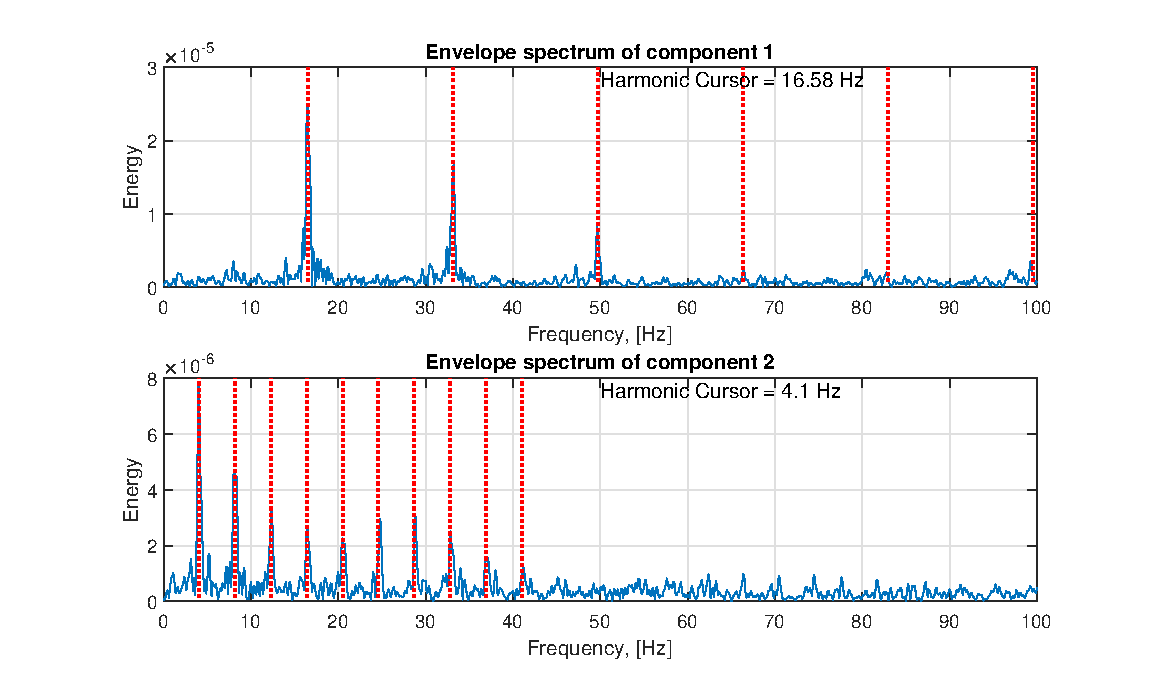
\includegraphics[width=\textwidth]{figs/env2.eps}
\caption{\textcolor{red}{Envelope spectra of recovered components.}}
\label{fig:NMF_env2}
\end{figure}

\section{Discussion}\label{disc}
The presented method properly separates and identifies both periodic impulsive components corresponding to different faults within the machine as well as the noise. Because of the multichannel approach, the information obtained from each channel can be merged. It allows to reconstruct each fault component correctly, even if partial information is missing in one of the classes. \textcolor{red}{However, the question can be posed about the reason behind the selection of this particular NMF version and not the basic "classic" NMF implementation.}

%nmf
\textcolor{red}{The $\beta$-HALS NMF has been used because of its performance. In particular, $\beta$-divergence is a different cost function than classically used mean square error. It provides better performance and stable convergence of optimization in comparison to the basic setup in the classic NMF algorithm. Additionally $\beta$-HALS NMF model is more robust to noise and achieves better fit than classic NMF model \cite{cichocki2008flexible}. There are several different divergences that can be used, but this one provides very good results for this type of analysis that requires “separative” properties of the matrix factorization algorithm. Another aspect is alternating least squares technique, which is more efficient for large-scale problems, especially using FCNNLS implementation (Fast Combinatorial Non-Negativity-constrained Least Squares) by Van Benthem and Keenan \cite{van2004fast}.}

\textcolor{red}{In the paper \cite{wodecki2019impulsive} authors demonstrated how unreliable is classic NMF. It is heavily influenced by randomly initiated state and very often produces incorrect results. This is the reason that authors were forced to employ Monte Carlo simulation to mitigate this effect and get the results as a probabilistic outcome of Monte Carlo. On the other hand, $\beta$-HALS NMF is in this context perfect and never fails in the quality of factorization (interpretation-wise: never fails in the correctness of component separation).}

Apart from its robustness, this method also exhibits certain limitations.  

%ograniczenie rozdzielności klastrów
The first one is connected to the selective capability of the spectrogram decomposition with NMF. The interpretation of this operation can be understood as a clustering technique in two ways: either as clustering short-time spectra according to their spectral structure or as clustering the subsignals corresponding to the elementary frequency bands according to their behavior as time series. In other words, one could interpret base matrix as centroids and encoding matrix as posterior probability structure (cluster assignment data), or the other way around. Regardless of this interpretation, the described limitation concerns the selectivity of the centroid structure. In other words, the efficiency of the component separation by NMF decreases when clusters start to overlap. 

%Ograniczenie precyzji spektrogramu
Another constraint concerns the resolution of used data representation. The entire concept is based on the idea that NMF is able to separate the components based on the factorization of the selected two-dimensional data representation (spectrogram in this case). As a consequence, the representation has to be precise enough to reveal all the behaviors, e.g. individual impulses. If this is not the case, it is required to either tweak the parameters to improve the resolution itself, or to select more appropriate representation (e.g. if the modulation frequency of the impulsive component is too high for the individual impulses to be observed, it is recommended to use the representation not related to the time domain, e.g. Cyclic Spectral Coherence \cite{wodecki2019impulsive}).

%ograniczenie artefaktów
User also has to be mindful of the way that the component identification is performed in section \ref{ident}. Hence it is based on the assessment of the modulation frequency of the individual components, it is not suitable for the evaluation of non-periodic components, especially artifacts, because they will not reveal any clear fundamental frequency.

%Czemu taki NMF
There are several different NMF algorithms developed over the years. One of the simplest implementations was proposed by Lee and Seung \cite{lee1999learning}. It imposes no additional constraints and has been successfully used by the authors in the past \cite{wodecki2019novel}. However, for such application it is lacking the precision and selectivity of class distinction. Due to such disadvantage, it was necessary to move towards an extended implementation equipped with additional features, and consequently more complicated. As a result, authors decided to use Generalized Hierarchical Alternating Least Squares Nonnegative Matrix Factorization with Beta-Divergence. Although its computational complexity is significantly higher, it allows to obtain more precise results. 

%ile klas
Another aspect to be aware of is the number of classes for NMF factorization. In the case of data presented in this article the choice was motivated by the composition: two damage components require two classes, with the third class meant for the signal background (one class is enough because of the consistency of the spectral structure of the background). The analysis of a real-life signal requires the experience in using NMF techniques and in general is either selected by hand in the process of trial and error or returned by some cluster evaluation criteria, such as Silhouette criterion \cite{rousseeuw1987silhouettes}. Too small number of classes causes unwanted partial mixing or even mixing of the components, which is a consequence of the fact that not every component has its own class to populate. On the other hand, too large number of classes causes the information of one component to be distributed among more than one class, which is a disadvantage from the point of view of further class identification. 

%dalsze prace
Authors anticipate several possibilities of expanding the functionality and robustness of the presented method. Firstly it is planned to modify the method of class identification so that it would be capable of the assessment of non-cyclic components as well as the cyclic ones. Secondly, the component reconstruction functionality will be modified towards the capability of receiving the contents of more than one class and synthesize a single component out of them. It will allow to deal with artifacts as well as impulsive non-cyclic noise. In both of those cases, the true component (either artifacts or impulsive noise) may require more than one NMF class, because the individual events (impulses produced by events randomly distributed in time, e.g. by a rock hitting the inside of a copper ore crusher \cite{wylomanska2016impulsive}) may not behave identically regarding their spectral structure.

\section{Conclusions}

In this paper, authors present a method for component separation based on multichannel vibration data. The information is distributed among the channels in a different way for each channel, which makes it complementary from the point of view of the individual channels. The idea of data fusion allows to obtain reliable results even in the presence of multiple cyclic components. In addition, the phase estimation procedure enables transforming obtained data structures back to the form of time series. As a result, the method allows to obtain signals related to periodic impulsiveness produced by individual local damages. \textcolor{red}{Presented method has been tested using two datasets: four-channel data describing healty gearbox with artificially introduced two different fault components, as well as dual-channel real-life data containing two faults occurring in the actual machine. In both cases presented method properly extracted the fault components from the signals allowing to identify their structure and especially frequencies of their occurrence, which allows to identify the faulty part of the machine. Data fusion aspect occurring during the reconstruction of the particular components played major role in obtaining much fuller information about the components than if the channels were to be analyzed as individual ones, which is the main conclusion speaking for using this method.}

\section*{Acknowledgments}
This activity has received funding from European Institute of Innovation and Technology (EIT), a body of the European Union, under the Horizon 2020, the EU Framework Programme for Research and Innovation. This work is supported by EIT RawMaterials GmbH under Framework Partnership
Agreement No. 17031 (MaMMa-Maintained Mine \& Machine).
\section*{References}

\bibliography{mybibfile}

\end{document}